\documentclass{article}
\usepackage[utf8]{inputenc}

\title{GEO1001 - Assignment 1 Report}
\author{Ondrej Veselý}
\date{21st September 2020}

\usepackage{natbib}
\usepackage{graphicx}

\begin{document}

\maketitle

\section*{Introduction}
For this assignment we used the data-set containing climate data measured in 5 locations within the town of Rijsenhout \citep{data}. The report is roughly subdivided into five sections related to each independent lesson (i.e. A1-4 + Bonus), with each section further split into a subsection for each corresponding question.

\newpage

\section{A1}

\subsection{Mean statistics}
\textit{
Compute mean statistics (mean, variance and standard deviation for each of the sensors variables), what do you observe from the results?
}\\

Answer.

\subsection{Temperature histograms}
\textit{
Create 1 plot that contains histograms for the 5 sensors Temperature values. Compare histograms with 5 and 50 bins, why is the number of bins important?
}\\

See Figure ~\ref{fig:1-2}.

\begin{figure}[!htb]
\centering
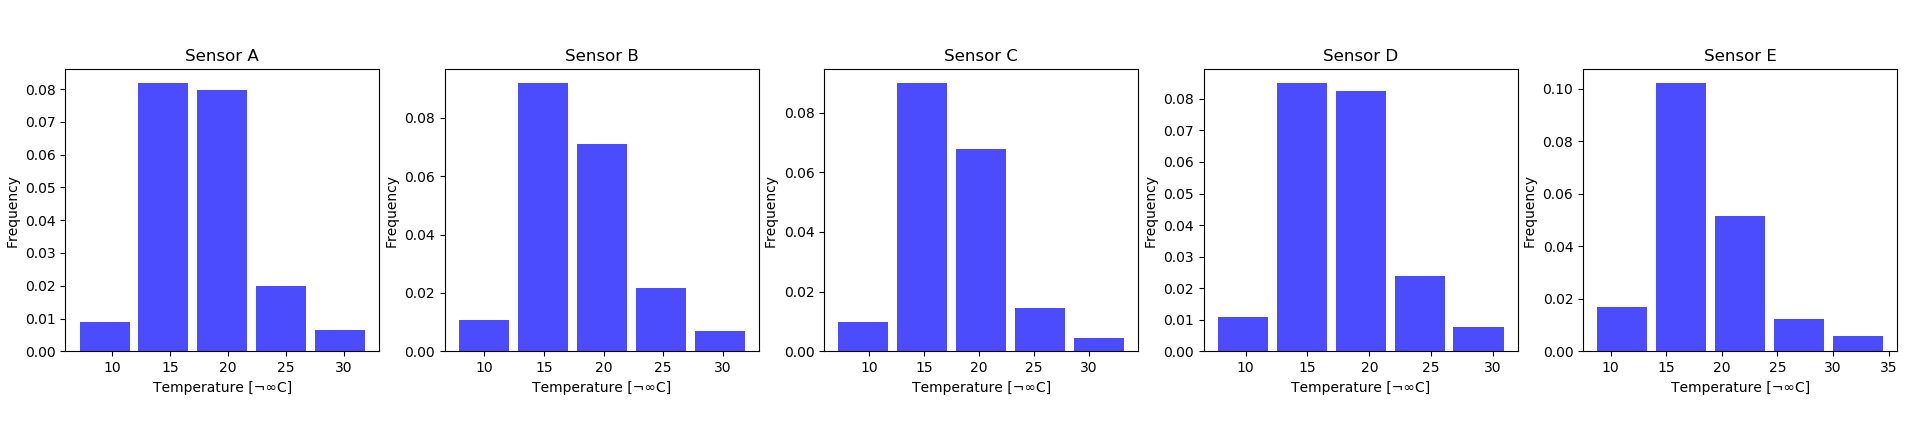
\includegraphics[width=\textwidth]{1-2-5_bins.png}
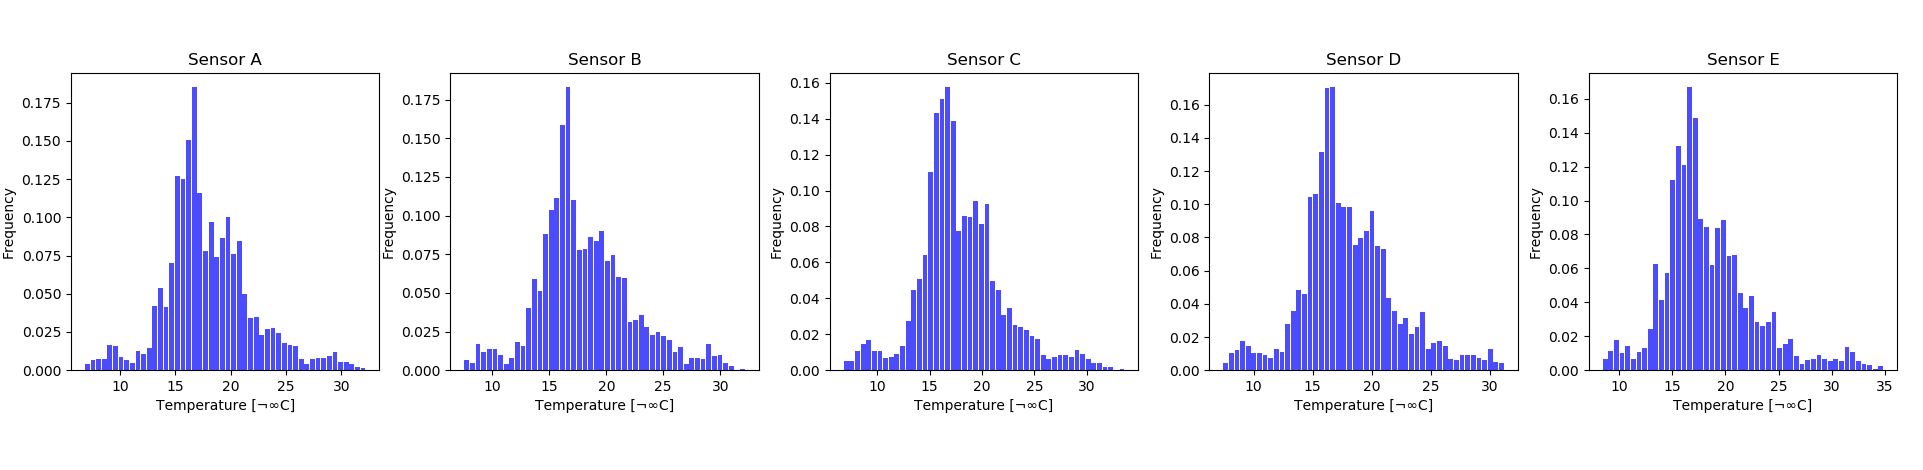
\includegraphics[width=\textwidth]{1-2-50_bins.png}
\caption{Comparison of different histogram binning values}
\label{fig:1-2}
\end{figure}

\newpage

\subsection{Temperature frequency polygons}
\textit{
Create 1 plot where frequency polygons for the 5 sensors Temperature values overlap in different colors with a legend.
}\\

See Figure ~\ref{fig:1-3}.

\begin{figure}[!htb]
\centering
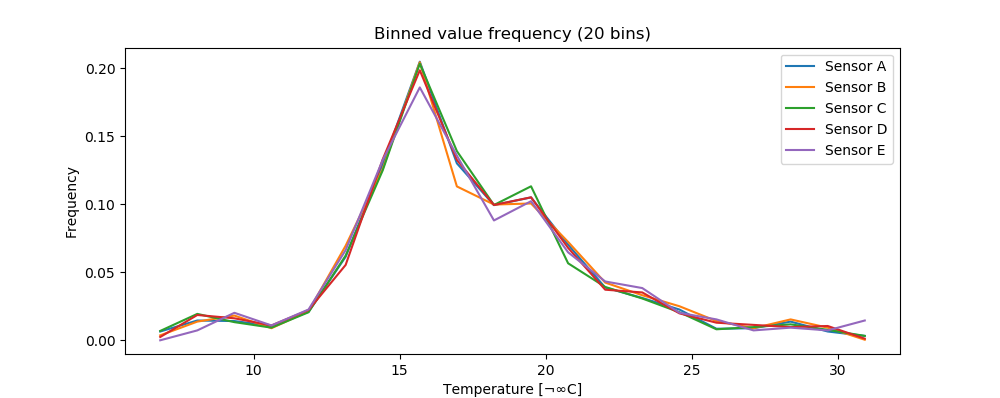
\includegraphics[width=\textwidth]{1-3-freq.png}
\caption{Temperature frequency polygons}
\label{fig:1-3}
\end{figure}

\subsection{Boxplots}
\textit{
Generate 3 plots that include the 5 sensors boxplot for: Wind Speed, Wind Direction and Temperature.
}\\

See Figure ~\ref{fig:1-4}

\begin{figure}[!htb]
\centering
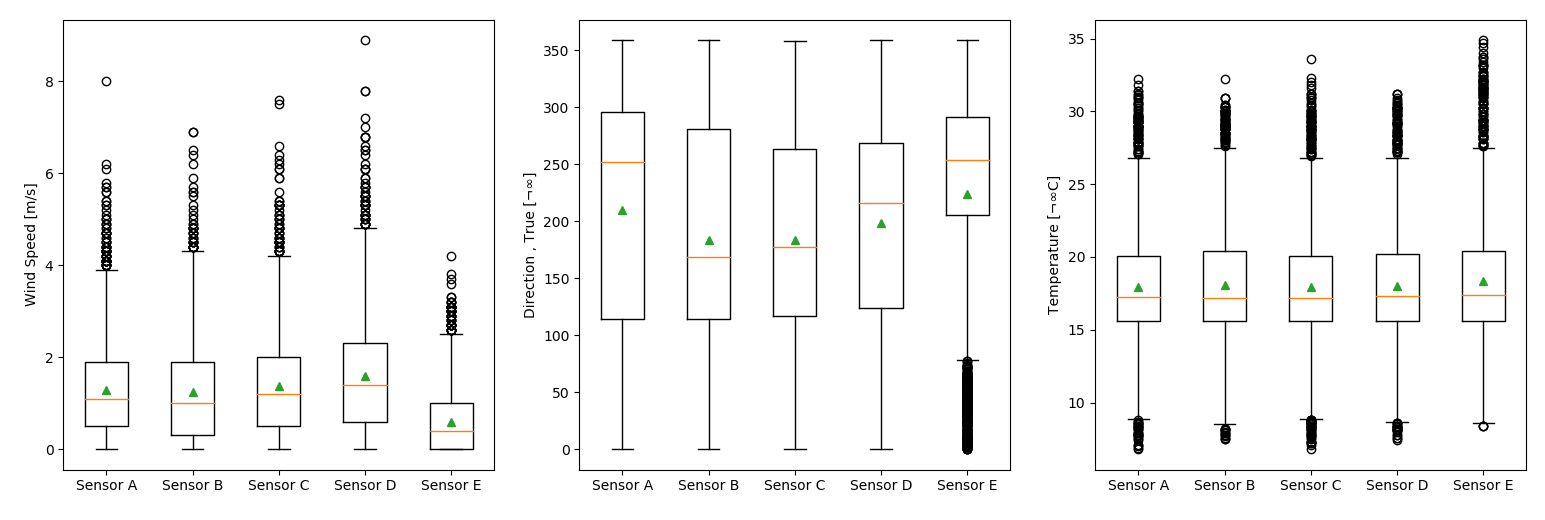
\includegraphics[width=\textwidth]{1-4-box.png}
\caption{Boxplots of Wind Speed, Direction and Temperature}
\label{fig:1-4}
\end{figure}

\newpage

\section{A2}

\subsection{Temperature distribution}
\textit{
Plot PMF, PDF and CDF for the 5 sensors Temperature values. Describe the behaviour of the distributions, are they all similar?
What about their tails?
}\\

See Figure ~\ref{fig:2-1}

\begin{figure}[!htb]
\centering
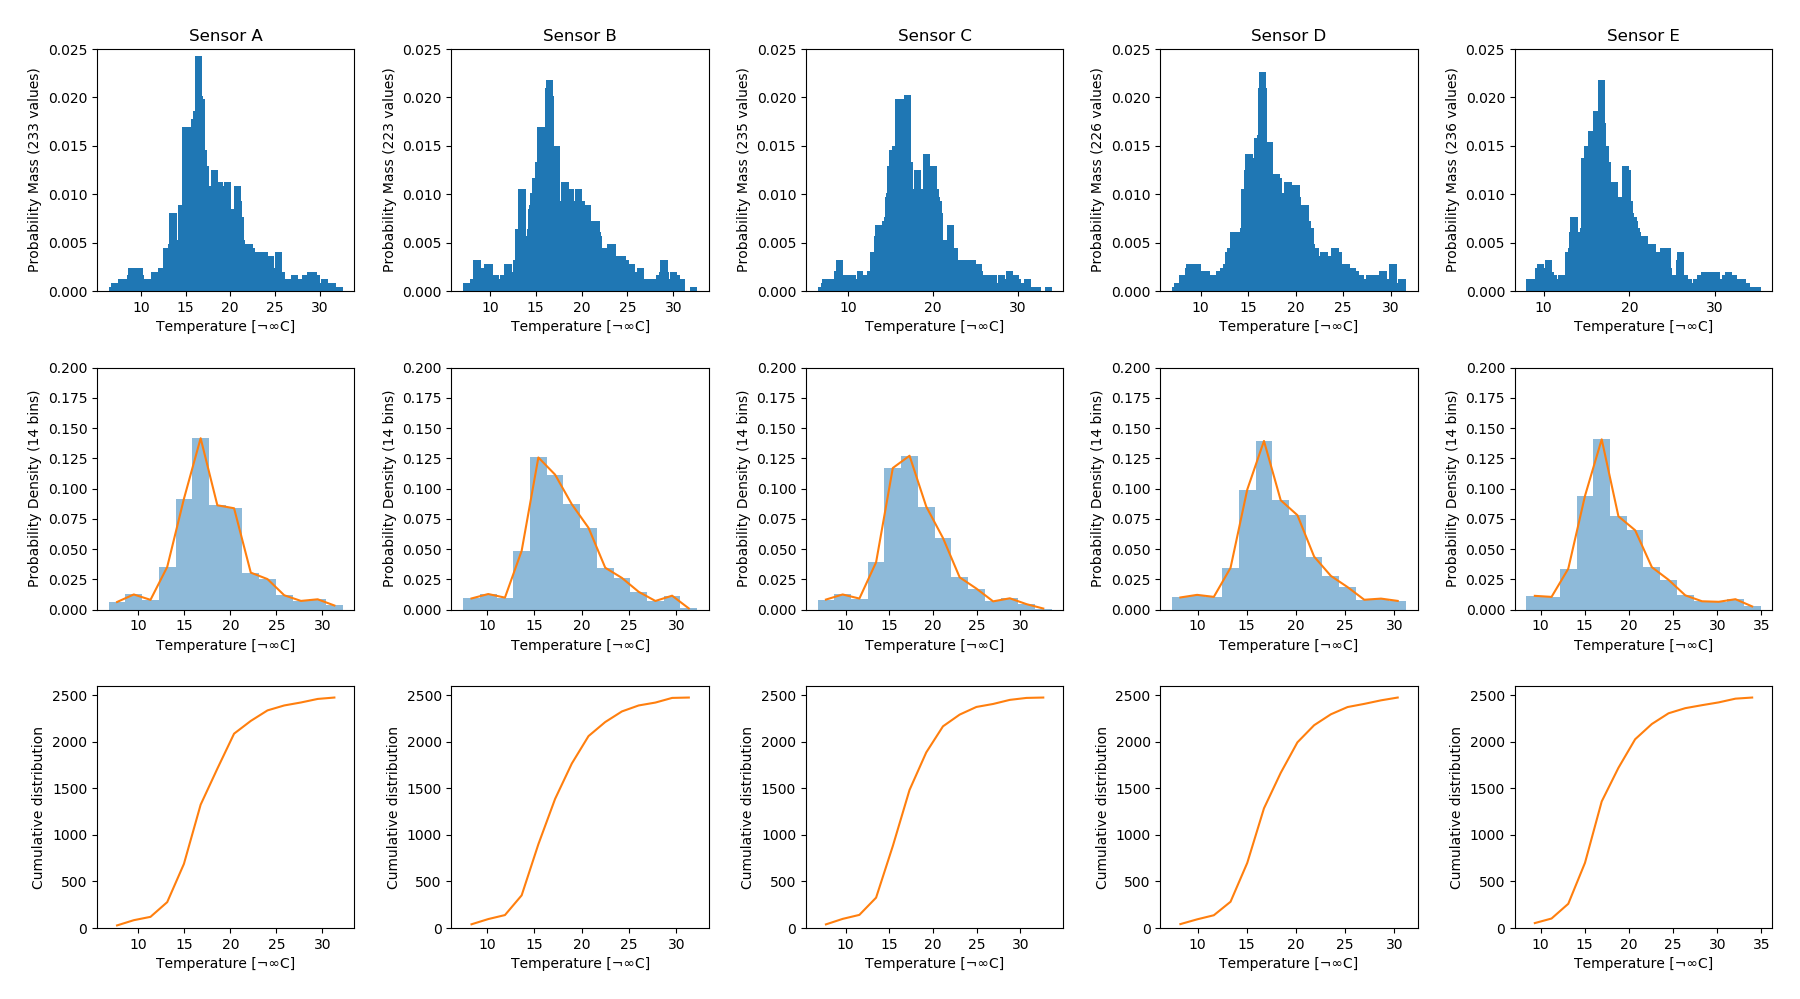
\includegraphics[width=\textwidth]{2-1-14_bins.png}
\caption{Probability mass, probability density and cumulative distribution functions of the temperature measurements}
\label{fig:2-1}
\end{figure}

\newpage

\section{A3}

\subsection{Correlation scatter-plot}
\textit{
Compute the correlations between all the sensors for the variables: Temperature, Wet Bulb Globe Temperature (WBGT), Crosswind Speed. Perform correlation between sensors with the same variable, not between two different variables; for example, correlate Temperature time series between sensor A and B. Use Pearson’s and Spearmann’s rank coefficients. Make a scatter plot with both coefficients with the 3 variables.
}\\


See Figure ~\ref{fig:3-1}

\begin{figure}[!htb]
\centering
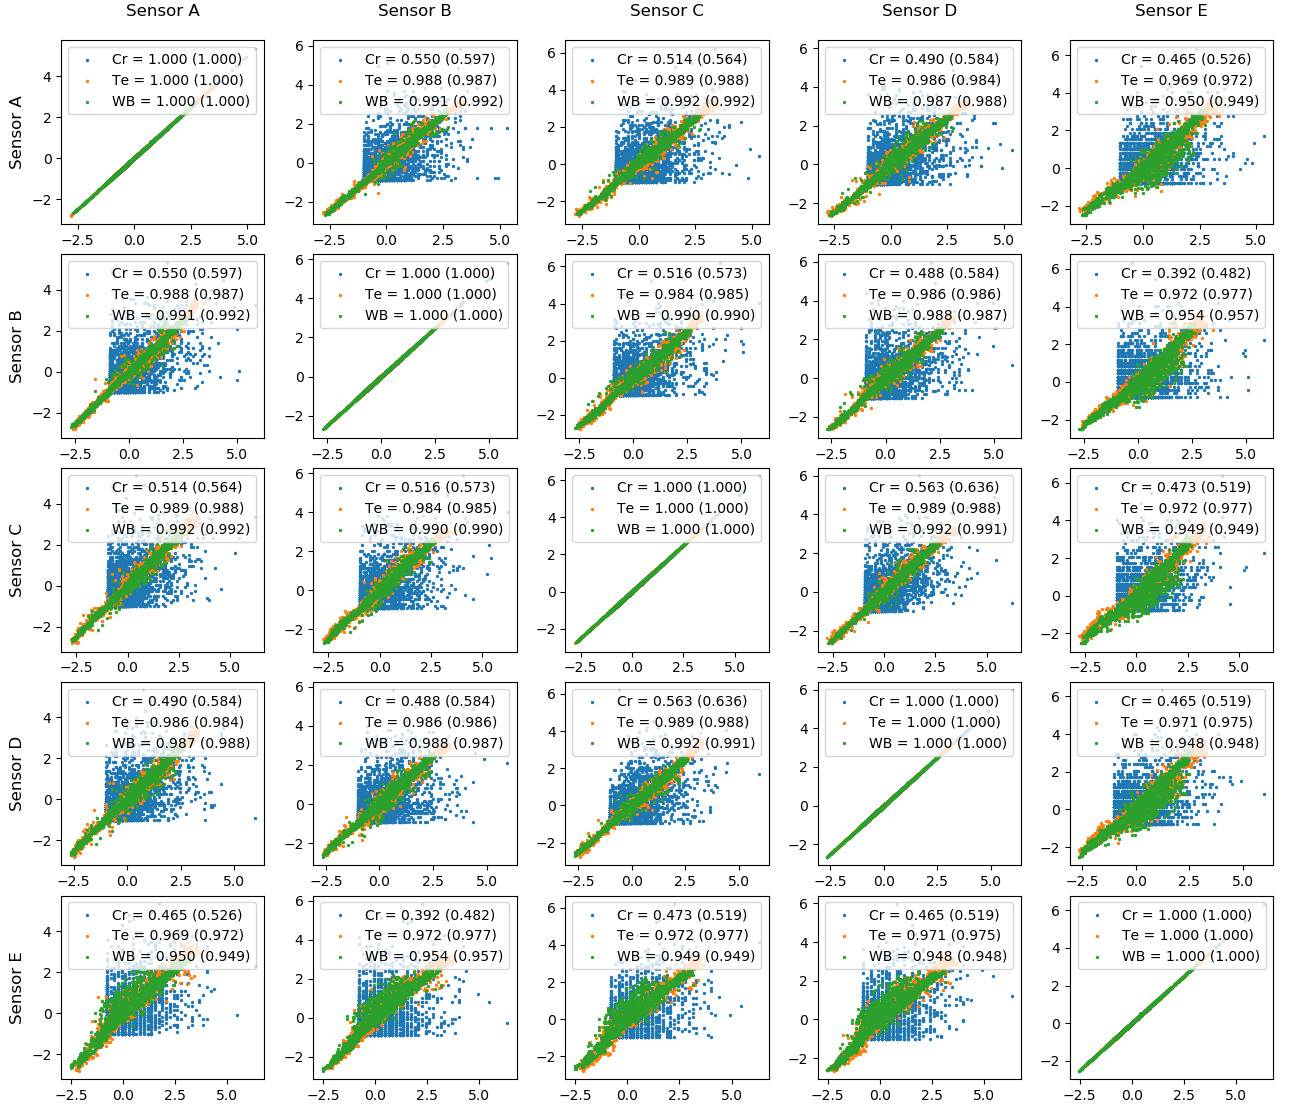
\includegraphics[width=\textwidth]{3-1-scatter.png}
\caption{Pearson (and Spearman) correlation ranks between all sensors measurements of Temperature(Te), Crosswind Speed(Cr) and WBGT(WB)}
\label{fig:3-1}
\end{figure}

\newpage

\subsection{Correlation conclusion}
\textit{
What can you say about the sensors’ correlations?
}\\

We observe very strong (\(r>0.9\)) correlations in Temperature and Wet Bulb Globe Temperature measurements in between all sensors.
The correlations between Crosswind Speed measurements are weak to moderate (\(0.4<r<0.6\)).
% That is however to be expected, since compered to the measured wind-speed, which may differ greatly with small differences in sensor placement, temperature is a much more of a macro-scale phenomena.


\subsection{Location hypothesis}
\textit{
If we told you that that the sensors are located as follows (Figure~\ref{fig:3-3}), hypothesize which location would you assign to each sensor and reason your hypothesis using the correlations.
}\\

\begin{figure}[!htb]
\centering
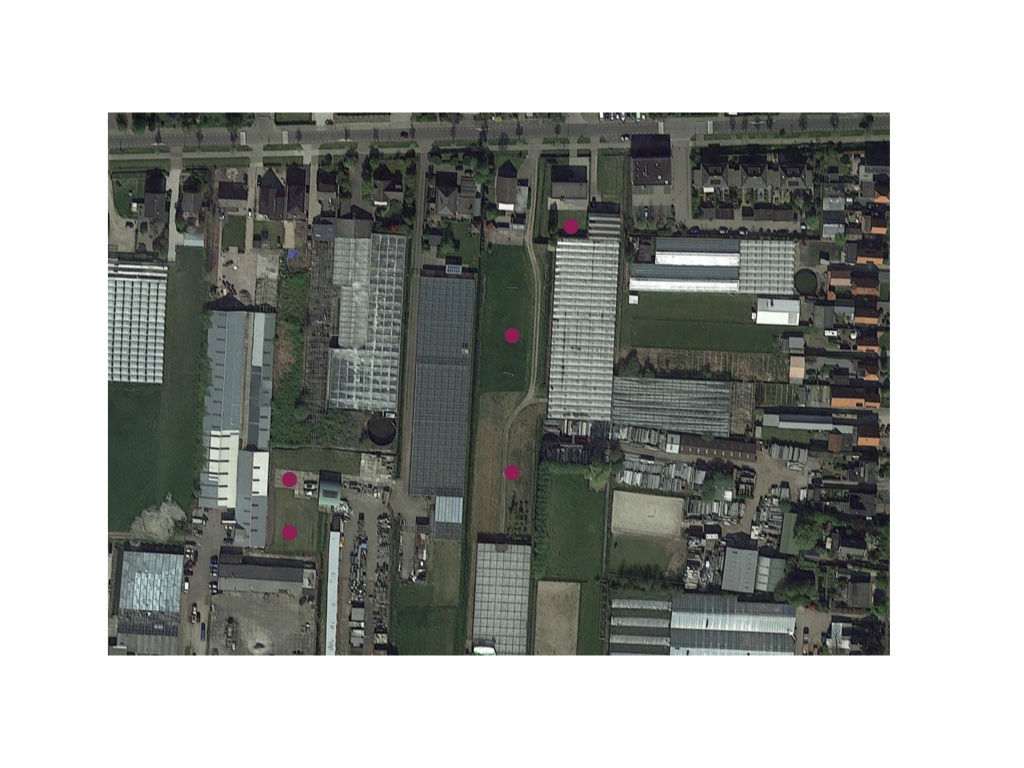
\includegraphics[width=\textwidth, trim={4cm 6cm 4cm 6cm}, clip]{3-3-map.png}
\caption{Situation map of the five sensors}
\label{fig:3-3}
\end{figure}

Two pairs on sensors have been each situated in close proximity to each other, or in very similar conditions. One sensor has been placed in a separate location. According to our hypothesis we should identify the two pairs by their stronger correlations and the one 'outlier' sensor by its weaker correlation to the rest of the group.
\\
\\The two mutually exclusive pairs with strongest correlations are:
\\ \quad Sensor C, D   \quad   \emph{Crosswind speed 0.563,   Temperature 0.989,   WBGT 0.992}
\\ \quad Sensor A, B   \quad   \emph{Crosswind speed 0.550,   Temperature 0.987,   WBGT 0.991}
\\
\\The remaining sensor E consistently has the lowest correlation with the rest of the sensors:
\\ \quad Sensor E, x   \quad   \emph{Crosswind speed \textless0.473,   Temperature \textless0.972,   WBGT \textless0.954}








\section{Conclusion}
``I always thought something was fundamentally wrong with the universe''

\begin{figure}[ht!]
\centering
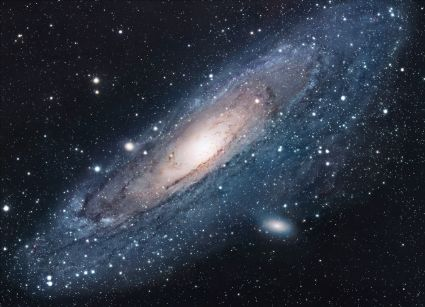
\includegraphics[scale=1.7]{universe}
\caption{The Universe}
\label{fig:universe}
\end{figure}

\bibliographystyle{plain}
\bibliography{references}
\end{document}
